%Made By Thomas Debelle
\documentclass{report}
\usepackage[a4paper, total={6in, 9in}]{geometry}
\usepackage[utf8]{inputenc}
\usepackage[francais]{babel}
\usepackage{graphicx}
\usepackage{graphics}
\usepackage[T1]{fontenc}
\usepackage{amsmath}
\usepackage{hyperref}
\usepackage{amssymb}
\usepackage{listings}
\usepackage{xcolor}
\usepackage{array}
\usepackage{float}
\usepackage{amsfonts}
\usepackage{fancyhdr}
\usepackage{titlesec}
\usepackage{xparse}
\usepackage{wrapfig}

\hypersetup{
    colorlinks=true,
    linkcolor=black,
    filecolor=magenta,
    urlcolor=cyan,
    pdftitle={Overleaf Example},
    pdfpagemode=FullScreen,
    }
\begin{document}


\begin{titlepage}
    \begin{figure}
        
\includegraphics[height = 2cm]{UCL_Logo.png}
        \label{fig:my_label}
    \end{figure}

    \hspace*{100cm}
    \centering
    \vspace*{7cm}

    {\Huge \textbf{Résumé de LELEC1370}}\\
    \vspace*{0.25cm}
    compilation du \today\\
    \vspace*{0.25cm}
    \Large{Thomas Debelle}\\

    \vspace*{9.5cm}
    {\Large Juin 2023}
\end{titlepage}


\tableofcontents
\newpage

\section*{Préface}

Bonjour à toi !\\

Cette synthèse recueille toutes les informations importantes données au cours, pendant les séances de tp et est améliorée grâce au note du Syllabus. Elle ne remplace pas le cours donc écoutez bien les conseils et potentielles astuces que les professeurs peuvent vous donner. Notre synthèse est plus une aide qui, on l'espère, vous sera à toutes et tous utile.\\

Elle a été réalisée par toutes les personnes que tu vois mentionnées. Si jamais cette synthèse a une faute, manque de précision, typo ou n'est pas à jour par rapport à la matière actuelle ou bien que tu veux simplement contribuer en y apportant tes connaissances ? Rien de plus simple ! Améliore la en te rendant \href{http://www.github.com/Tfloow/Q4_EPL}{ici} où tu trouveras toutes les infos pour mettre ce document à jour. (\textit{en plus tu auras ton nom en gros ici et sur la page du github})\\

Nous espérons que cette synthèse te sera utile d'une quelconque manière ! Bonne lecture et bonne étude.


\chapter{Cours 1}
\section{Les bases}

Tout d'abord, il existe 2 types de courant appelé \textbf{Direct Current} ou \textit{DC} et \textbf{Alternating Current} ou \textit{AC}. Le courant direct est continu tandis que le courant \textit{AC} varie dans le temps comme montré ci-contre.\\
\begin{figure}[H]
	\centering
	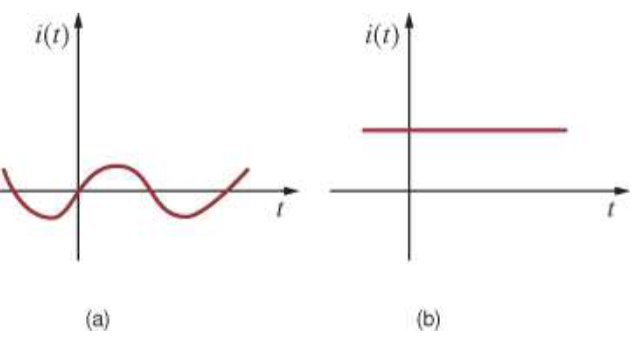
\includegraphics[width=.3\textwidth]{img/ACDC.png}
	\caption{Gauche: courant AC \quad Droite: courant DC}
\end{figure}
La tension vaut la variation d'énergie selon la charge ou autrement dit: 
\begin{equation}
v = \frac{dw}{dq}
\end{equation}
La puissance vaut la tension par le courant ou:
\begin{equation} \label{eqn:p}
p = vi = \frac{dw}{dq}\frac{dq}{dt}
\end{equation}
Finalement, l'énergie est une différence de puissance en fonction du temps:
\begin{equation}
\Delta w = \int_{t_1}^{t_2}p dt = \int_{t_1}^{t_2} vi dt
\end{equation}
Quelques conventions:
\begin{itemize}
\item Source de tension nulle = court circuit
\item Source de courant nulle = circuit ouvert
\item Le sens du courant "rentre" dans la borne + d'un générateur de tension.
\end{itemize}
\subsubsection{Puissance dissipée}
Pour connaitre la puissance dissipée dans une résistance, on utilise d'abord la formule fondamentale d'une résistance:
\begin{equation}
v(t) = R i(t)
\end{equation}
Ainsi, en utilisant \ref{eqn:p} on trouve:
\begin{equation} \label{eqn:pr}
p(t) = vi(t) = \frac{v^2(t)}{R} = Ri^2(t)
\end{equation}

\subsubsection{Loi des noeuds de Kirchoff}
La somme des courants de tous les noeuds a pour résultat 0. Autrement dit, tout courant qui apparait disparait quelque part.

\subsubsection{Loi des mailles de Kirchoff}
Dans un circuit électrique, on peut dessiner des \textit{mailles} ou des sortes de carrés. En tournant dans un sens, on fait la somme des tensions (\textit{faire attention au sens des tensions}) on obtient une somme nulle.

\subsubsection{Sources multiples - Diviseur de tension}
On peut simplifier un circuit et sommer des sources de tension en additionnant leur tension. On utilise également la règle des diviseurs de tension pour les résistances:
\begin{equation}
\begin{cases}
\parallel \rightarrow R_{new} = \frac{1}{\frac{1}{R_1}+\frac{1}{R_2}}\\
\text{série} \rightarrow R_{new} = R_1 + R_2
\end{cases}
\end{equation}

\subsubsection{Mise en parallèle et sources multiples}
Les sources de courant en parallèle peuvent être sommé pour les simplifier et n'en avoir qu'une seule source de courant.

\subsubsection{Équivalent Thévenin Norton}
On peut simplifier une alimentation d'un circuit via les circuits de Thévenin et Norton. Thévenin est composé d'une source de tension et d'une résistance en série tandis que Norton a une source de courant et une résistance en parallèle.\\
Les choses importantes à noter sont:
\begin{equation}
\begin{cases}
R_{Th} = R_{No}\\
I_{sc} = \frac{V_{R}}{R_{Th}}\\
v_{oc} = R_{Th}i_{sc}
\end{cases}
\end{equation}
 
\begin{figure}[H]
\centering
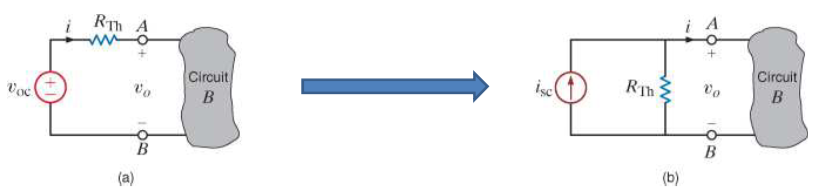
\includegraphics[width = 10cm]{img/ThNo.png}
\caption{Illustration du passage de Thévenin à Norton}
\end{figure}
Pour trouver la résistance $R_{Th}$ on met en \textit{court-circuit} les générateurs de tensions et en \textit{circuit ouvert} les générateurs de courant. Ensuite, on enlève la résistance et on regarde à ses bornes les \textit{résistances} et on trouve donc \textit{l'équivalent des résistances}. On peut faire cela uniquement avec des générateurs \textbf{non commandés}.\\

Pour trouver le \textit{courant de Norton} et la \textit{tension de Thévenin} (on est \textbf{obligé} de passer par cette étape en premier avec des \textit{sources commandées}). Pour \textit{Thévenin} on met notre résistance en \textit{circuit ouvert} et on trouve le voltage à ses bornes.\\
Pour \textit{Norton} on met notre résistance en \textit{court-circuit} et on trouve le courant circulant dans ce fil.

\subsubsection{Conseil Norton Thévenin}
Lorsqu'on travaille avec des courants, on utilise la loi des \textit{noeuds} et une fois qu'on a toutes les équations, on utilise la loi des \textit{mailles} qui permet d'utiliser nos courants et tout simplifier.\\

\subsubsection{Dualité étoiles-triangle}
Dans un circuit électrique, on peut faire face à des arrangements de résistances en \textit{triangle} qui sont compliqués à transformer en \textit{résistance équivalente}. 
\begin{figure}[H]
\centering
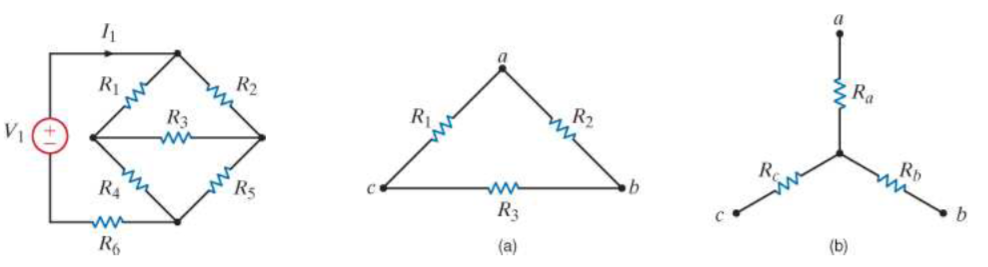
\includegraphics[width=7cm]{img/triangleEtoile.png}
\caption{Passage d'une forme de triangle à une forme d'étoiles}
\end{figure}
Les équations sont:
\begin{align}
R_1 &= \frac{R_a R_b + R_b R_c + R_a R_c}{R_b}\\
R_a &= \frac{R_1 R_2}{R_1 + R_2 + R_3}
\end{align}



\chapter{Cours 2}
\section{Suite des bases}
\subsubsection{Thévenin avec sources dépendantes}
Pour trouver $R_{Th}$ on va rajouter au borne connectant l'autre circuit une source de tension. Puis on détermine les tensions à borne ouverte et le courant en \textit{court-circuit}.

\subsubsection{Transfert maximal de puissance}
Pour trouver la puissance maximale dans une résistance, on peut faire varier le courant et donc le voltage. Ici, on a réalisé un diviseur résistif très simple pour démontrer la formule de puissance de résistance donné par \ref{eqn:pr}, on obtient donc ceci dans notre circuit:
\begin{equation}
\frac{\partial}{\partial R_2} \biggl(\frac{V^2 R_2}{(R_1 + R_2)^2}\biggl) = 0
\end{equation}

\begin{figure}[H]
\centering
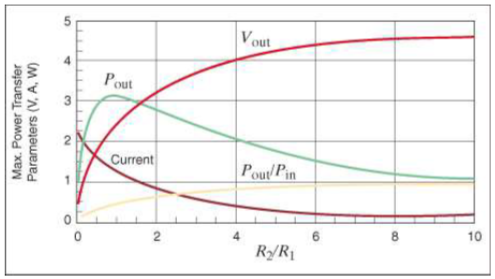
\includegraphics[width=6.5cm]{img/maxPuissance.png}
\caption{Graphique montrant l'évolution de la puissance dans une résistance}
\end{figure}

\subsubsection{Le quadripole à 2 accès}
\begin{wrapfigure}{r}{.45\textwidth}
\centering
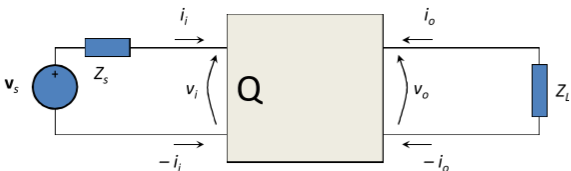
\includegraphics[width=6.5cm]{img/quadri2.png}
\caption{Schéma classique d'un quadripole à 2 accès}
\end{wrapfigure}
Le quadripole à 2 accès se reposent sur 2 principes, il faut qu'il n'y ait aucune source indépendante interne $\rightarrow$ donc passif. Il faut également n'avoir que 2 accès, c'est à dire que la somme des entrées est nulle. Pour simplifier, il faut qu'on ait une entrée et sortie comprenant le même courant (voir schéma ci-contre).\\
Le but de cette représentation est une simplification de circuit. De plus, même si ce circuit n'est pas linéaire, on fait des petites variations autour d'une valeur rendant approximativement le circuit linéaire.\\

Ce type de quadripole peut être réalisé de 4 manières différentes détaillées ci-dessus.
\begin{figure}[H]
\centering
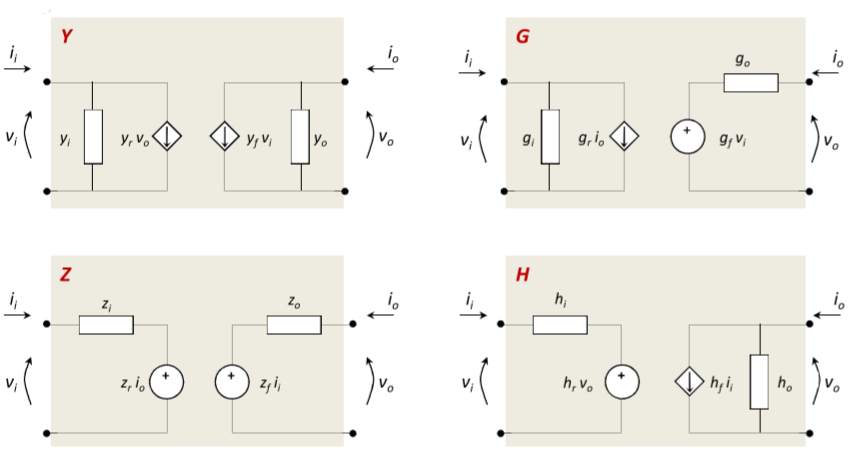
\includegraphics[width=6cm]{img/YZGH.png}
\caption{Les 4 types de quadripoles}
\end{figure}
On peut facilement représenter ces différents systèmes via des matrices détaillants le système
%insérer la matrice

\subsection{L'amplificateur opérationnelle}
L'amplificateur opérationnelle ou \textit{ampli op} est un composant qu'on retrouve abondamment en électronique. 

\subsubsection{Montage inverseur}
\begin{equation}
\frac{v_o}{v_s} ~= -\frac{R_2}{R_1}
\end{equation}

\chapter{Signaux sinusoïdales et phaseurs}
\section{Circuits en régime sinusoïdal}

\subsection{Circuit RC: rappel}
Dans cette partie, on s'intéressera surtout au circuit \textbf{RC}, il est donc bon de rappeler différentes formules:
\begin{align}
I_C(t) &= C \frac{dV_C(t)}{dt}\\
V_R(t) &= RI(t)\\
RC \frac{dV_C(t)}{dt} &= -(V_C(t)-V_S(t))\label{eq:RCsinus}
\end{align}

\begin{figure}[H]
\centering
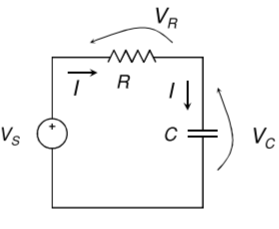
\includegraphics[width=5cm]{img/RCsinus.png} \label{img:RCsinus}
\caption{Circuit RC en régime sinusoïdal}
\end{figure}

Il est à noter que l'équation \ref{eq:RCsinus} est une équation propre au circuit de la figure \ref{img:RCsinus}. Il est bon de remarquer que \textit{maintenant}, les courants et tension sont \textit{dépendantes du temps}. La \textit{constante de temps} est $\tau = RC$ et apparait dans la résolution de \textit{l'équation différentielle}.

\subsection{Circuit LC}
Voici les formules pou les circuits LC. (\textit{note}: on dirait que notre source de courant est une source de courant \textit{commandé} mais c'est bien une source de courant \textbf{non-commandé})
\begin{align}
V_L(t) &= L \frac{dI_L(t)}{dt}\\
V_L(t) &= GI_G(t)\\
GL \frac{dI_L(t)}{dt} &= -(I_L(t)-I_S(t))\label{eq:LCsinus}
\end{align}

\begin{figure}[H]
\centering
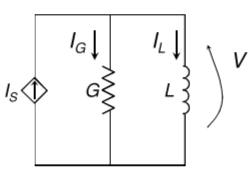
\includegraphics[width=4.6cm]{img/LCsinus.png} \label{img:LCsinus}
\caption{Circuit LC en régime sinusoïdal}
\end{figure}

Il est à noter que l'équation \ref{eq:LCsinus} est une équation propre au circuit de la figure \ref{img:LCsinus}. La \textit{constante de temps} est $\tau = GL$

\subsection{Régime sinusoïdal}
Quelques notions à bien comprendre:
\begin{itemize}
\item La phase est établi par l'observateur car c'est lui qui définit "\textit{le début de la sinusoïdale}
\item Un cosinus est un sinus \textit{déphasé} de $\frac{\pi}{2}$
\end{itemize}

\subsubsection{Analyse circuit RC}
Si on a une source de courant sinusoïdale:
\begin{align}
V_s(t) &= V_p cos(\omega t)\\
\omega_0 &= \frac{1}{\tau} = \frac{1}{RC}\\
\frac{1}{\omega_0}\frac{dV_c(t)}{dt} + V_c(t) &= V_p cos(\omega t) \label{eq:RCdiff}
\end{align}

L'équation \ref{eq:RCdiff} correspond à l'équation différentielle et à pour solution:

\begin{equation} 
\begin{cases}
V_C(0) = 0\\
V_C(t) = \frac{V_p}{\textcolor{blue}{\sqrt{1 + \frac{\omega^2}{\omega_0^2}}}} \Bigl[\textcolor{brown}{-cos(\varphi)e^{-\frac{t}{\tau}}} + \textcolor{green}{cos(\omega t + \varphi)} \Bigl] \label{eq:RCsol}
\end{cases} 
\end{equation}
L'équation \ref{eq:RCsol} nous indique plusieurs choses:
\begin{enumerate}
\item La partie en \textcolor{blue}{bleu} nous montre une atténuation du signal.
\item La partie en \textcolor{brown}{brun} nous montre une partie \textit{transitoire} dû à la capacité qui se charge doucement avant d'arriver à un état stable.
\item La partie en \textcolor{green}{vert} est le \textit{déphasage} du signal qui est créé par le caractère "\textit{dérivateur}" d'une capacité
\end{enumerate}

%finir de clarifier les 2 dernières slides de cette sous-section

\subsection{Les Phaseurs}
On utilise des \textbf{phaseurs} pour des circuits:
\begin{itemize}
\item \textit{linéaires}
\item  ne possédant \textit{qu'une source indépendante}
\item on a une source de fréquence $\omega/ 2\pi$
\item le circuit est \textit{en régime}
\end{itemize}

Donc tous les autres \textit{courants dépendants} ont
\begin{itemize}
\item une \textit{forme} ressemblant à la source
\item la \textit{même fréquence}
\item une \textit{amplitude différente} 
\item une \textit{phase différente}
\end{itemize}
Seulement si cela est respecté, alors on peut utiliser les \textbf{phaseurs}:
\begin{align}
\textbf{V} &= V_M e^{j\psi_V}\\
\textbf{I} &= I_M e^{j\psi_I}
\end{align}
En électricité, on représente le nombre complexe par $j$. $\psi$ représente les phases.\\
L'utilisation des \textit{phaseurs} vient de l'idée de la \textit{formule d'Euler} où quand on ajouter une partie imaginaire, cela n'affecte pas la partie \textit{réelle}. Donc on peut faire ceci:
\begin{equation}
\begin{cases}
A cos(\omega t + \varphi) \rightarrow A cos(\omega t + \varphi) + j A sin(\omega t + \varphi) \qquad -\frac{\pi}{2}  \geq \varphi \geq \frac{\pi}{2} \\
A cos(\omega t + \varphi) \rightarrow \bigr[ Ae^{j\varphi} \bigr]e^{j\omega t}
\end{cases} 
\end{equation}
Ici, la deuxième équation utilise des \textit{phaseurs} (mis entre parenthèses, l'utilisation de phaseurs va simplifier notre notation surtout en dérivée et intégrale:
\begin{align}
\frac{d}{dt}\bigr[ Ae^{j\varphi} \bigr]e^{j\omega t} &= \bigr[ j \omega Ae^{j\varphi} \bigr]e^{j\omega t} \\
\int \bigr[ Ae^{j\varphi} \bigr]e^{j\omega t} &= \bigr[ \frac{1}{j \omega} Ae^{j\varphi} \bigr]e^{j\omega t}
\end{align}

Il est important de se rappeler que lorsqu'on travaille en \textit{complexe}, multiplier par $j$ reviens à faire une rotation \textit{anti-horlogé} de $\frac{\pi}{2}$.

%clarifier la fin

\subsection{Analyse de circuits}
Passer en phaseur est un opération \textbf{linéaire} donc toutes les lois de \textit{Kirchoff} et théorèmes de la \textit{théorie des circuits} restent \textbf{valables}.

\begin{center}
\begin{tabular}{|c|c|c|c|}
\hline
Élément & Résistance & Inductance & Capacité\\
\hline 
Paramètre & $\textbf{Z} = R$ & $\textbf{Z} = j\omega L$ & $\textbf{Z} = \frac{1}{j \omega C}$\\
$\textbf{Z} = \frac{1}{\textbf{Y}}$ & $\textbf{Y} = \frac{1}{R}$ & $\textbf{Y} = \frac{1}{j \omega L}$ & $j \omega C$ \\
\hline 
Équation constitutive & $V = \textbf{Z}I$ & $V = \textbf{Z}I$ & $V = \textbf{Z}I$\\
 & $I = \textbf{Y}V$ & $I = \textbf{Y}V$ & $I = \textbf{Y}V$\\
\hline
\end{tabular}
\end{center}

Pour des \textbf{dipôles}:
\begin{center}
\begin{tabular}{|c|c|}
\hline
\textbf{Impédance} d'un dipôle & \textbf{Admittance} d'un dipôle\\
\hline
$\textbf{V} = \textbf{ZI}$ & $\textbf{I} = \textbf{YV}$\\
\hline
$\textbf{Z} = \frac{\textbf{V}}{\textbf{I}} = \frac{|\textbf{V}|}{|\textbf{I}|}e^{j(arg(\textbf{V})-arg(\textbf{I})} = \frac{V}{I} e^{j{(\psi_V-\psi_I)}}$ & $\textbf{Y} = \frac{\textbf{I}}{\textbf{V}} = |\textbf{Y}|e^{j(arg(\textbf{Y}))} = Y e^{j{(\varphi)}}$\\
\hline
\end{tabular}
\end{center}

On a différente notation pour $\textbf{Z}$:
\begin{align}
\textbf{Z} &= |\textbf{Z}|e^{j arg(\textbf{Z})} = Z e^{j\varphi} \qquad \text{représentation polaire}\\
\textbf{Z} &= R +jX \qquad \text{représentation cartésienne}
\end{align}
\begin{wrapfigure}{r}{.5\textwidth}
\centering
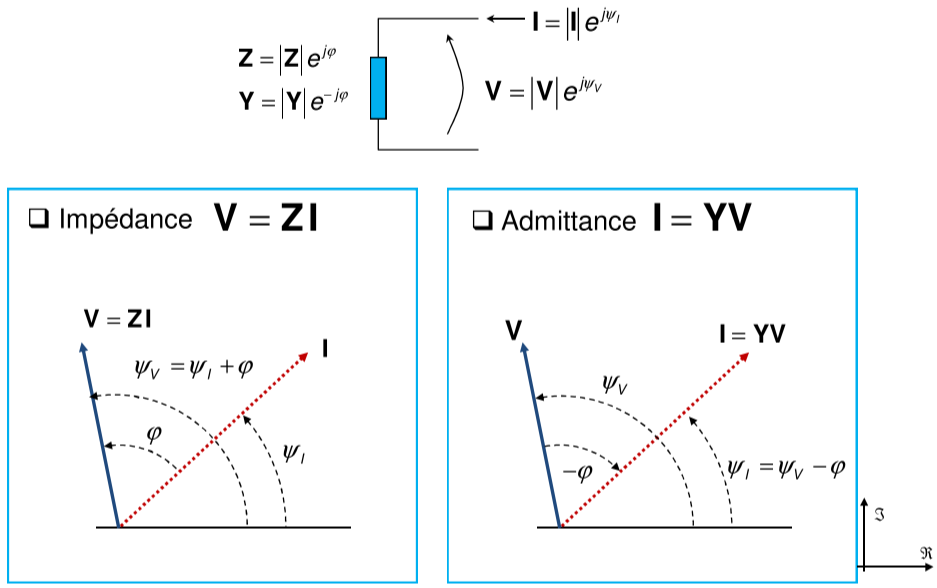
\includegraphics[width=7cm]{img/impedance.png}
\end{wrapfigure}

R est la \textit{résistance} et X la \textit{réactance}. Si cette dernière est \textbf{négative}, on a affaire à une \textit{capacité}. Si elle est \textbf{positive}, il s'agit d'une \textit{inductance}

Donc on voit clairement que notre vecteur \textbf{Z} a une composante \textit{complexe} et \textit{réelle}. Et cela vaut de même pour le vecteur \textbf{Y}.

\subsubsection{Impédance de résistance pure}
\begin{itemize}
\item $\textbf{V} = R \textbf{I}$ et donc $\textbf{Z} = R$
\item Tension en phase: $\varphi = 0 \rightarrow \textbf{V} = RI_Me^{j\psi_I}$
\item Admittance: $\textbf{Y} = G = \frac{1}{R}$ 
\end{itemize}

\subsubsection{Impédance d'inductance pure}
\begin{itemize}
\item $\textbf{V} = j \omega L \textbf{I}$ et donc $\textbf{Z} = j \omega L$
\item Tension en \textbf{avance} sur le courant: $\varphi = \frac{\pi}{2} \rightarrow \textbf{V} = \omega L I_M e^{j(\psi_I + \frac{\pi}{2})}$
\item Admittance: $\textbf{Y} = jB = \frac{1}{j \omega L}$ 
\end{itemize}


\subsubsection{Impédance de capacité pure}
\begin{itemize}
\item $\textbf{I} = j \omega C \textbf{V}$ et donc $\textbf{Y} = j \omega C$
\item Tension en retard sur le courant: $\varphi = \frac{-\pi}{2} \rightarrow \textbf{I} = \omega C V_M e^{\psi_V + \frac{\pi}{2}}$
\item Impédance: $\textbf{Z} = jX = \frac{1}{j \omega C}$ 
\end{itemize}
Attention à bien remarquer l'utilisation d'une impédance au lieu d'une admittance comme précédemment.

\subsubsection{Même dipôle}
\begin{figure}[H]
\centering
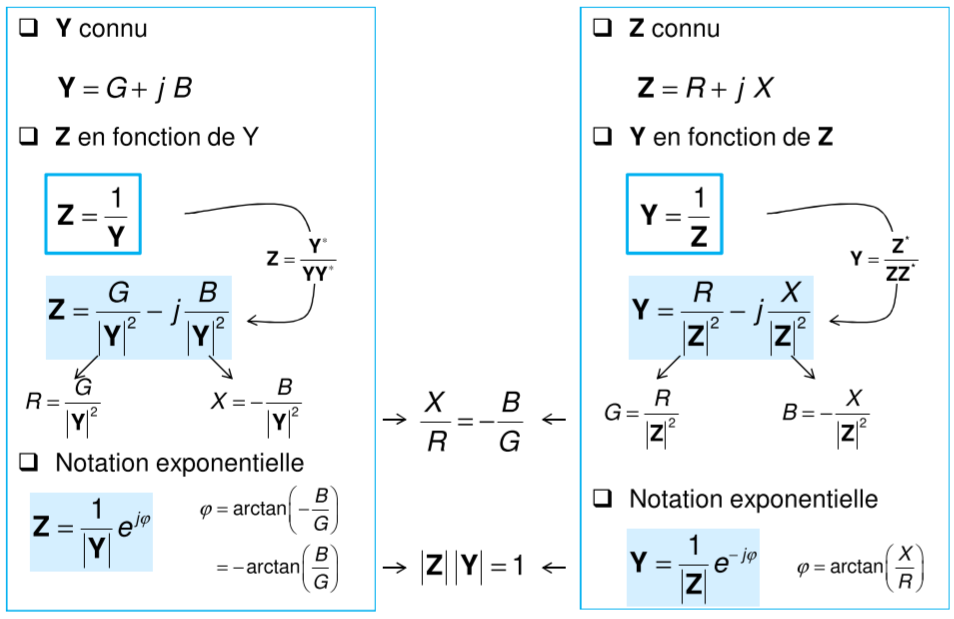
\includegraphics[width=7cm]{img/memeDipole.png}
\end{figure}

\subsection{Admittance équivalente à une impédance}
A une \textcolor{red}{fréquence précise}, tout dipôle en série peut être remplacé par un dipôle en parallèle.\\

En effet, il suffit de recréer le même vecteur. Dans le cas en \textbf{série}, on impose le courant donc:
\begin{align}
\textbf{$V_{R}$} &= |\textbf{Z}|cos(\varphi) \textbf{I} \rightarrow \textbf{Z} = R\\
\textbf{$V_{L}$} &= |\textbf{Z}|sin(\varphi) \textbf{I} \rightarrow \textbf{Z} = \omega L \\
\end{align}
Et dans le second cas, on impose la tension au borne:
\begin{align}
\textbf{I} &= \textbf{V} \textbf{Y}\\
\textbf{$I_{R}$} &= \frac{1}{|\textbf{Z}|}cos(\varphi) \textbf{V} \rightarrow \textbf{Y} = \frac{1}{\textbf{Z}}\\
\textbf{$I_{L}$} &= \frac{|\textbf{Z}|}{sin(\varphi)} \textbf{V} \rightarrow \textbf{Y} = \frac{1}{\omega L} 
\end{align}
Il faut bien se rendre compte que cet équivalent est uniquement valable pour une \textcolor{red}{même fréquence}. Car le $|\textbf{Z}|$ varie ainsi que le déphasage $\varphi$. \\
Pour faire la différence quand on a des graphes comme ci-dessous, on peut voir que à basse fréquence (donc quasi DC) aucun courant ne passe dans la capacité pour un circuit en parallèle. Cela implique qu'on a pas de déphasage car tout le courant passe dans 	la résistance. De plus, l'impédance est quasi constante. (\textit{on peut prouver un équivalent la même chose pour le circuit en série})

\begin{figure}[H]
\centering
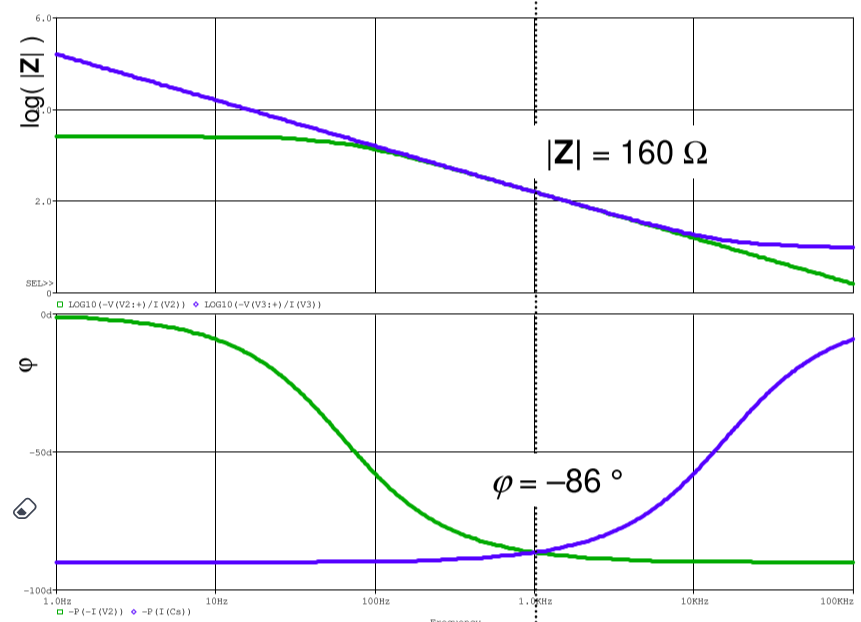
\includegraphics[width=7cm]{img/EquivalentRC.png}
\caption{En \textcolor{blue}{bleu} le circuit en série, en \textcolor{green}{vert} le circuit en parallèle}
\end{figure}

\subsection{Addition Impédance}
Comme dit au début du chapitre, on conserve toutes les lois classiques des circuits en courant continu. Cela implique que:
\begin{itemize}
\item Pour les impédances:
	\begin{itemize}
	\item On additionne simplement les impédances en série.
	\item On réalise la formule $\frac{1}{\frac{1}{Z_1} + ... + \frac{1}{Z_n}}$ pour des impédances en parallèle.
	\end{itemize}
\item Pour les admittances:
	\begin{itemize}
	\item On réalise la formule $\frac{1}{\frac{1}{Z_1} + ... + \frac{1}{Z_n}}$ pour des admittances en série.
	\item On additionne simplement les admittances en parallèle.
	\end{itemize}
\end{itemize}
Cette \textit{dualité} impédances admittances est très utile et simplifie de nombreux calculs pour les circuits \textit{AC}.

\subsection{Thévenin et Norton}
On fait les mêmes démarches qu'en \textit{DC}, il faut faire attention aux impédances complexes et les sources de courants et tension qui sont des \textit{phaseurs}.

\chapter{Comportement des circuits en domaine fréquentielle}
Nous avons déjà vu que la \textit{fréquence} influence notre \textit{impédance} et \textit{phase}.

\section{Diagramme de Bode}
Le Diagramme de Bode est une façon conventionnelle de représenter un circuit selon une évolution de la fréquence. Ce type de graphe utilise des axes logarithmiques avec en axe \textbf{X} la fréquence et en axe \textbf{Y} notre valeur d'intérêt (ici, un courant)

\begin{figure}[H]
\centering
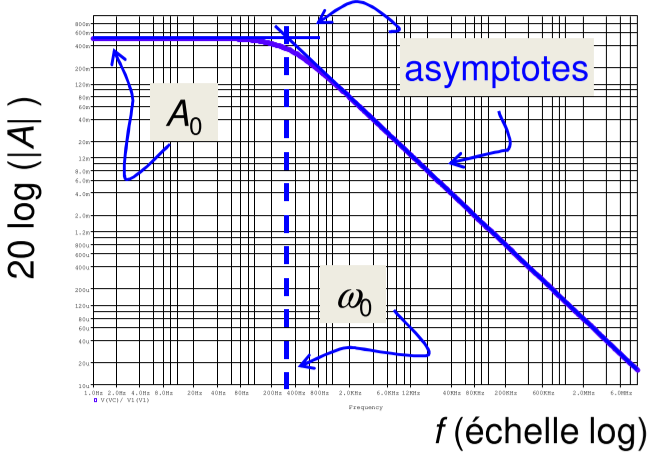
\includegraphics[width=6.5cm]{img/BodeEx.png}
\caption{Exemple pour $\textbf{A} = A_0 \frac{1}{1 + \frac{j \omega}{\omega_0}}$}
\end{figure}


\end{document}


